% 結果の章（数値は 図/values.tex と 図/tab_*.tex から。手で書かない）

% ============================================================
\chapter{主な検定}\label{ch:primary}

\begin{table}[H]
\centering\small
\caption{主な検定 P：2020 年以降・範囲の中の発表で、2〜60 取引日のドリフトを \code{chrono\_ridge} と統制・固定効果で回帰した結果}
\label{tab:primary}
\begin{tabular}{@{}lr@{}}
\toprule
点数が 1 標準偏差高いときのドリフトの差 & \V{Pcoef} bp \\
95\% 信頼区間 & [\V{Plo}, \V{Phi}] bp \\
$t$（反応日ごとにまとめた標準誤差） & \V{Pt} \\
片側 $p$ & \V{Pp} \\
置換（同じ反応日の中で 1,000 回）の片側 $p$ & \V{Pperm} \\
発表の数（反応日の数） & \V{Pn}（\V{Pdates}） \\
決定係数の増分 & \V{Prtwo} ポイント \\
\midrule
判定 & \textbf{\V{Pverdict}} \\
\bottomrule
\end{tabular}
\end{table}

\begin{keybox}[結果]
事前登録の判定の基準（片側 $t$ の $p < 0.05$、かつ置換の片側 $p < 0.05$）を両方とも満たし、仮説は\textbf{支持}された。ChronoGPT＋リッジの点数が 1 標準偏差高い発表は、発表をはさむ 2 日の反応・SUE・売上の驚き・発表の前の値動き・規模・業種と時期の固定効果を統制したうえで、その後 2〜60 取引日の IWM との超過リターンが平均 \V{Pcoef} bp 高かった。置換の $p$ の \V{Pperm} は、1,000 回の置換のどれも実際の係数を超えなかったことを示す（1,000 回の置換で出せる最小の値）。
\end{keybox}

\begin{itemize}
\item \textbf{大きさ}：1 標準偏差あたり約 0.8\% は、60 取引日（約 3 か月）の超過リターンとしては小さくない。ただし決定係数の増分は \V{Prtwo} ポイントで、個々の発表のドリフトの変動のごく一部しか説明しない。一つ一つの発表の予測は外れることが多い。
\item \textbf{2021 年以降}（生存者バイアスの小さい期間、事前登録の頑健性）：係数 \V{Rcoef} bp（$t$ = \V{Rt}、片側 $p$ \V{Rp}、発表 \V{Rn} 件）。同じ向きで、やや大きい。
\end{itemize}

% ============================================================
\chapter{副次の検定と比較}\label{ch:secondary}

\section{ほかの点数のドリフト}

\begin{table}[H]
\centering\small
\caption{副次の検定：2〜60 日のドリフトの回帰（族ごとに Holm の補正。判定には使わない）}
\label{tab:secondary}
\tabin{secondary}
\end{table}

\begin{itemize}
\item \textbf{学習ありの点数}は、どれも正の係数を持った。ChronoGPT の 26 層目（\code{chrono\_mid\_ridge}）は Holm の補正の後も有意、FinBERT の追加学習（\code{finbert\_ft}）は補正の前は 5\% で有意、補正の後は 10\% の水準だった。
\item \textbf{学習なしの点数}のうち、辞書は負（$t$ は約 $-2$）、FinBERT はほぼゼロだった。
\item \textbf{gpt-4o-mini の期間}（2024 年以降）では、学習なしの gpt-4o-mini（語調＋見通し＋ガイダンス）が最も大きく、重みを学習したもの、ChronoGPT＋リッジも、どれも Holm の補正の後に有意だった。
\end{itemize}

\section{比較の表}

\begin{table}[H]
\centering\small
\caption{2020 年以降：係数（bp/SD）と、括弧の中は $t$}
\label{tab:compare2020}
\tabin{compare_2020}
\end{table}

\begin{table}[H]
\centering\small
\caption{2024 年以降（gpt-4o-mini の点数がそろう発表）：係数（bp/SD）と、括弧の中は $t$}
\label{tab:compare2024}
\tabin{compare_2024}
\end{table}

\begin{figure}[H]
\centering
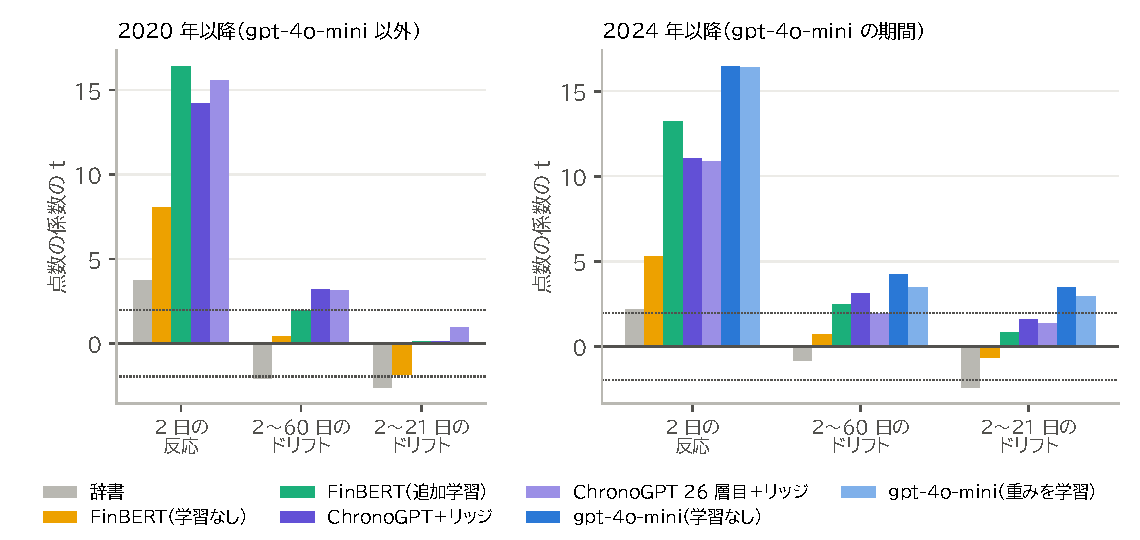
\includegraphics[width=\linewidth]{compare.pdf}
\caption{点数の係数の $t$。点線は $\pm 1.96$。}
\label{fig:compare}
\end{figure}

\begin{itemize}
\item \textbf{2 日の反応}は、どの点数でも強く説明できた。\SP{} の実験と同じで、学習ありのモデル（FinBERT の追加学習、ChronoGPT＋リッジ）と gpt-4o-mini が特に強い。
\item \textbf{2〜21 日}では、ChronoGPT＋リッジの係数はほぼゼロで、gpt-4o-mini（2024 年以降）だけが有意に正だった。辞書は負だった。
\item つまり、ChronoGPT＋リッジの 2〜60 日のドリフトは、主に \textbf{22〜60 日目}に生じている（\ref{sec:explore} 節で確かめた）。
\end{itemize}

% ============================================================
\chapter{時価総額加重との対決}\label{ch:portfolio}

事前登録の副次の 4：毎月末、範囲の中の会社のうち、直近 92 日以内の最新の発表の点数の上位 20\% を浮動株時価総額で加重したポートフォリオと、範囲の全社を浮動株時価総額で加重したもの（比べる相手）を比べた。

\begin{table}[H]
\centering\small
\caption{月次の超過リターン（上位 20\% − 範囲の全社）と Newey--West の $t$（ラグ 3）}
\label{tab:portfolio}
\begin{tabular}{@{}lrrrrrr@{}}
\toprule
 & \multicolumn{2}{c}{費用 0\%} & \multicolumn{2}{c}{片道 0.3\%} & \multicolumn{2}{c}{片道 0.5\%} \\
\cmidrule(lr){2-3}\cmidrule(lr){4-5}\cmidrule(lr){6-7}
 & 月次 & $t$ & 月次 & $t$ & 月次 & $t$ \\
\midrule
ChronoGPT＋リッジ（\V{Mstart}〜\V{Mend}、\V{Mmonths} か月） & \V{Mexa} & \V{Mta} & \V{Mexb} & \V{Mtb} & \V{Mexc} & \V{Mtc} \\
gpt-4o-mini（重みを学習、\V{Gstart}〜\V{Gend}、\V{Gmonths} か月） & \V{Gexa} & \V{Gta} & \V{Gexb} & \V{Gtb} & \V{Gexc} & \V{Gtc} \\
\bottomrule
\end{tabular}
\end{table}

\begin{figure}[H]
\centering
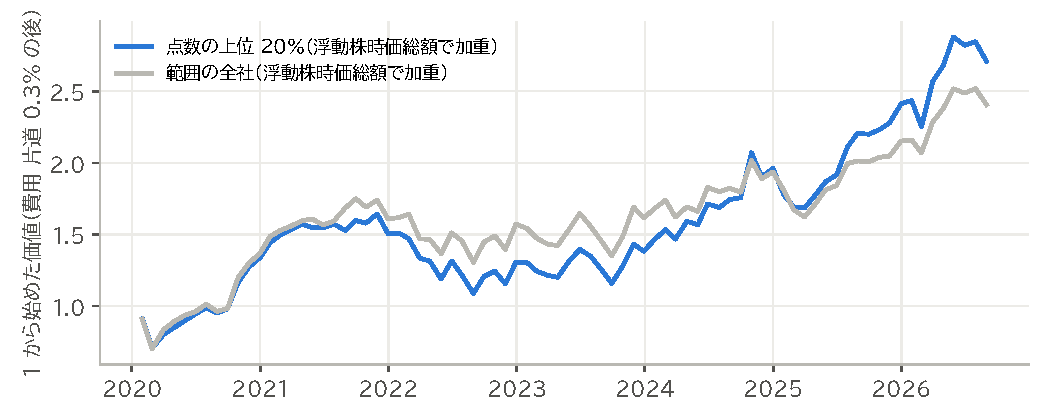
\includegraphics[width=\linewidth]{portfolio.pdf}
\caption{ChronoGPT＋リッジの上位 20\% と、範囲の全社（2020 年 1 月を 1、片道 0.3\% の費用の後）。}
\label{fig:portfolio}
\end{figure}

\begin{figure}[H]
\centering
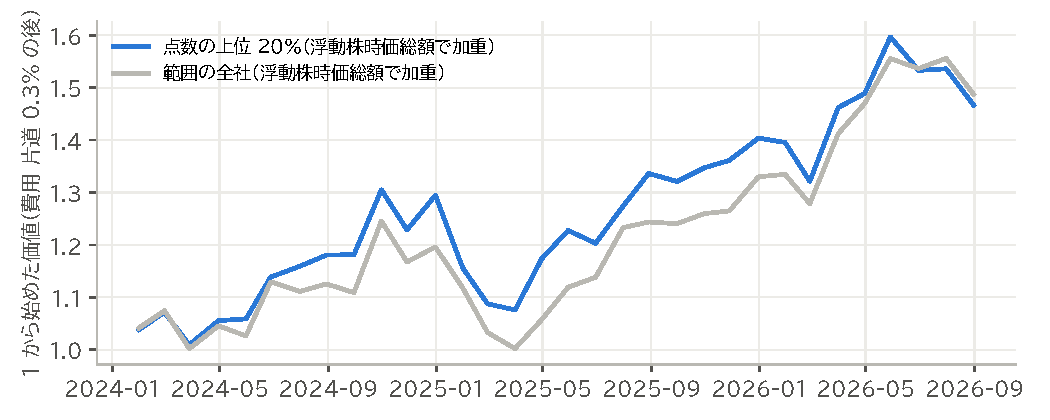
\includegraphics[width=\linewidth]{portfolio_gpt.pdf}
\caption{gpt-4o-mini（重みを学習）の上位 20\% と、範囲の全社（2024 年 1 月を 1、片道 0.3\% の費用の後）。}
\label{fig:portfoliogpt}
\end{figure}

\begin{itemize}
\item ChronoGPT＋リッジの上位 20\% は、費用の前で月 \V{Mexa}、片道 0.3\% の費用の後で月 \V{Mexb}、比べる相手を上回ったが、有意ではなかった（$t$ = \V{Mtb}）。上位 20\% の月の回転率は平均 \V{Mturn}。
\item gpt-4o-mini（重みを学習）は、V{Gmonths} か月と短く、費用の後はほぼゼロだった。
\item 回帰で見えた予測の力（\chapref{ch:primary}）が、浮動株時価総額で加重した月次のポートフォリオの差として、有意に現れるほどの大きさではなかった。回帰は発表を等しく扱い、業種と時期の影響を除くが、ポートフォリオは規模で加重し、市場全体の変動の中で比べる。
\item 両方のポートフォリオの月次の平均リターン（上位 20\% が \V{Mtop}、範囲の全社が \V{Mall}）は、今も上場している会社だけを選んだ生存者バイアスで高く出ている。意味があるのは差だけである。
\end{itemize}

% ============================================================
% BLM の資産の推移（事前登録の追記 1。検定はせず報告だけ）
\chapter{BLM の資産の推移}\label{ch:blm}

事前登録の追記 1（どの株価の反応も計算する前に追加）：四半期（3・6・9・12 月）・半年（6・12 月）・1 年（12 月）ごとにリバランスする BLM の比率で、2015 年 12 月末と 2023 年 12 月末をそれぞれ 1 とした資産の推移を作った（\code{blm\_paths.py}）。

\begin{itemize}
\item 範囲：各リバランスの日に小型株の範囲にいて、直近 252 日のうち 126 日以上の株価がある会社。
\item 見通し：その日以前に反応日がある、直近 92 日以内の最新の発表の点数を正規スコアにした。BLM は実験 7・9 と同じ形（$\delta = 2.5$、$\tau = 0.025$、He--Litterman の $\Omega$、IC $= 0.05$）で、見通しの大きさは保有期間に合わせた（日次で IC × $\sigma_{\text{日}}$ × $z / \sqrt{h}$）。共分散は直近 252 日の Ledoit--Wolf。事前の TE の上限は年 3\%（校正しない）。
\item 比べる相手：同じ範囲を浮動株時価総額で加重したもの。両方から、売買した額の片道 0.3\% を引いた。
\item \textbf{検定はしない}（事前登録の通り、報告だけ）。
\end{itemize}

\section{2015 年末から}

\begin{table}[H]
\centering\small
\caption{2015 年 12 月末を 1 とした資産の推移（2026 年 9 月末まで）。年率と相手との差は年率、実現の TE は年率、回転率はリバランス 1 回あたり}
\label{tab:blm2015}
\tabin{blm_2015}
\end{table}

\begin{figure}[H]
\centering
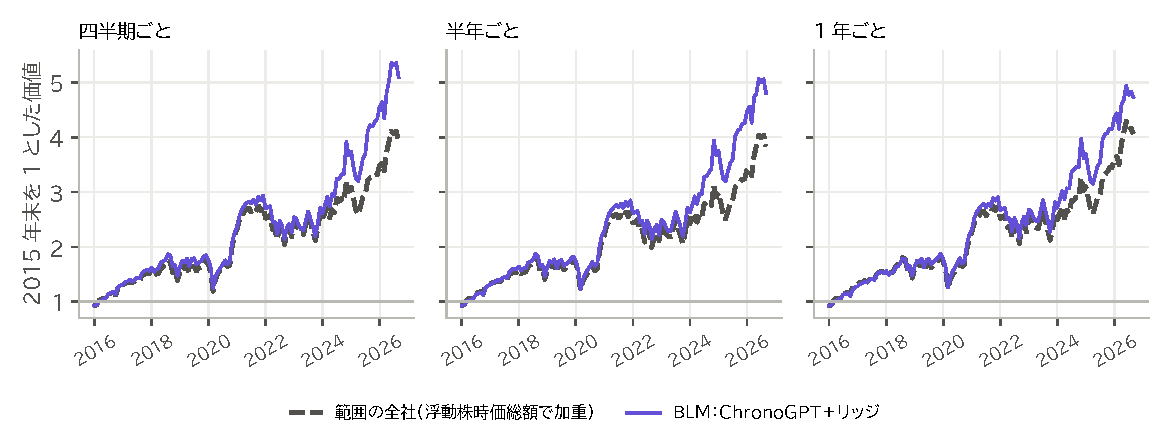
\includegraphics[width=\linewidth]{blm_2015.pdf}
\caption{2015 年末を 1 とした推移。BLM は ChronoGPT＋リッジの見通し。}
\label{fig:blm2015}
\end{figure}

\section{2023 年末から}

\begin{table}[H]
\centering\small
\caption{2023 年 12 月末を 1 とした資産の推移（2026 年 9 月末まで、約 2 年 9 か月）}
\label{tab:blm2023}
\tabin{blm_2023}
\end{table}

\begin{figure}[H]
\centering
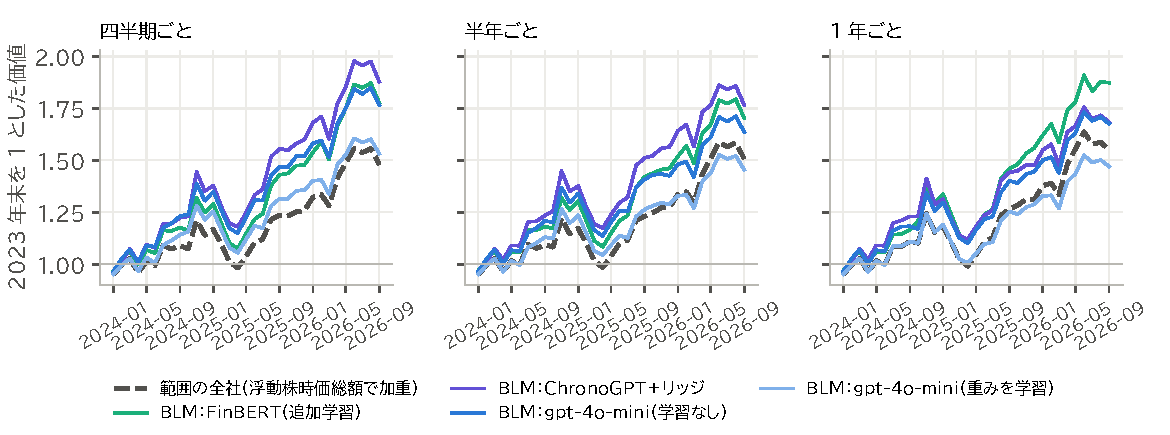
\includegraphics[width=\linewidth]{blm_2023.pdf}
\caption{2023 年末を 1 とした推移。gpt-4o-mini（重みを学習）は 2024 年の第 1 四半期から点数があり、それ以前の日は見通しなし（範囲の比率）。}
\label{fig:blm2023}
\end{figure}

\section{読み方}

\begin{itemize}
\item \textbf{2015 年末から}：ChronoGPT＋リッジの BLM は、3 つのリバランスの頻度のどれでも、比べる相手を年率で上回った（四半期 \V{B2015quarterchronoridgeex}、半年 \V{B2015halfchronoridgeex}、1 年 \V{B2015yearchronoridgeex}）。最終の値は、四半期で \V{B2015quarterchronoridge}、比べる相手は \V{B2015quarterband}。ただし、\figref{fig:blm2015} のとおり、差の多くは 2023 年以降に開いた。2016〜2022 年は、ほぼ同じ動きだった。
\item \textbf{2023 年末から}：ChronoGPT＋リッジ、FinBERT（追加学習）、gpt-4o-mini（学習なし）の BLM は、どの頻度でも比べる相手を上回った。gpt-4o-mini（重みを学習）は、四半期ではわずかに上回り、半年・1 年では下回った。期間が約 2 年 9 か月と短く、1 年ごとのリバランスは 3 回しかない。
\item \textbf{資産の水準}は、2 本とも生存者バイアスで高く出ている（比べる相手の年率が 13〜17\%）。特に 2015 年からの推移は、範囲の会社の約半分が欠ける時期を含む。意味があるのは、同じ会社の範囲での 2 本の差である。
\item \textbf{実現の TE} は年 3〜7\% 程度で、多くは事前の上限（3\%）を超えた。事前の TE を校正しなかったこと（事前登録で決めた）と、最適化の多くの回で解の精度が「不正確」（\code{optimal\_inaccurate}）と報告されたことによる。不正確と報告された解も、そのまま使った（\code{results/blm\_paths.json} の \code{status}）。
\item \textbf{回帰との関係}：主な検定の予測の力（\chapref{ch:primary}）は、BLM の小さな傾き（TE 数\%）の中で、比べる相手との差として現れた。一方、規模で加重した上位 20\% の月次のポートフォリオ（\chapref{ch:portfolio}）では、有意な差にならなかった。どちらも 1 回の実行の結果であり、BLM の差は検定していない。
\end{itemize}


% ============================================================
\chapter{探索}\label{ch:explore}

\section{事前登録した探索：ドリフトを正解に学習したリッジ}

同じ ChronoGPT のベクトルのリッジを、2 日の反応ではなく 2〜60 日のドリフト（窓が閉じたものだけ）を正解にして学習すると、係数は \V{Ecoef} bp（$t$ = \V{Et}）で、予測の力はなかった。ドリフトはばらつきが大きく、それを直接に学習するには標本が足りない。2 日の反応で「読み取りの強さ」を学び、それがドリフトを予測するかを見る事前登録の設計（主な検定）のほうが、うまくいった。

\section{事前登録の後の探索}\label{sec:explore}

以下は、主な検定の結果を見た後に追加した分析で、\textbf{事前登録にない}。コードは \code{explore.py}、結果は \code{results/explore.json}（どちらも \code{experiments/S1\_smallcap\_drift/} の下）。置換の検定はしていない。試した分析はここに書いたものだけだが、これらを結論の根拠にはしない。

\subsection{点数の 5 分位}

\begin{table}[H]
\centering\small
\caption{点数の 5 分位ごとの、IWM との超過リターンの平均（bp、上下 1\% で丸めた。統制なし）}
\label{tab:quintiles}
\tabin{quintiles}
\end{table}

ChronoGPT＋リッジでは、2〜21 日の差は小さく、22〜60 日に上位と下位の差が開く。gpt-4o-mini では 2〜21 日にも差がある。どちらも上位 2 つの分位が高く、下位が低い。

\subsection{22〜60 日だけの窓・モメンタム・規模}

\begin{table}[H]
\centering\small
\caption{事前登録の後の探索の回帰（係数 bp/SD、括弧の中は $t$。統制と固定効果は主な検定と同じ）}
\label{tab:explore}
\begin{tabular}{@{}lll@{}}
\toprule
分析 & 点数 & 結果 \\
\midrule
22〜60 日だけの窓（2020 年以降） & ChronoGPT＋リッジ & \V{Xdays2260chronoridgec}（\V{Xdays2260chronoridget}） \\
 & FinBERT（追加学習） & \V{Xdays2260finbertftc}（\V{Xdays2260finbertftt}） \\
 & 辞書 & \V{Xdays2260dictionaryc}（\V{Xdays2260dictionaryt}） \\
22〜60 日だけの窓（2024 年以降） & gpt-4o-mini（学習なし） & \V{Xdays2260gptgptc}（\V{Xdays2260gptgptt}） \\
 & gpt-4o-mini（重みを学習） & \V{Xdays2260gptgptridgec}（\V{Xdays2260gptgptridget}） \\
\midrule
過去 1 年のモメンタムを統制に追加（2〜60 日） & ChronoGPT＋リッジ & \V{Xplusmomentumchronoridgec}（\V{Xplusmomentumchronoridget}） \\
 & FinBERT（追加学習） & \V{Xplusmomentumfinbertftc}（\V{Xplusmomentumfinbertftt}） \\
 & gpt-4o-mini（学習なし、2024 年以降） & \V{Xplusmomentumgptgptc}（\V{Xplusmomentumgptgptt}） \\
 & gpt-4o-mini（重みを学習、2024 年以降） & \V{Xplusmomentumgptgptridgec}（\V{Xplusmomentumgptgptridget}） \\
\midrule
規模で 2 つに分ける（2〜60 日） & 浮動株時価総額の小さい半分 & \V{Xbysizesmallerc}（\V{Xbysizesmallert}） \\
 & 大きい半分 & \V{Xbysizelargerc}（\V{Xbysizelargert}） \\
\bottomrule
\end{tabular}
\end{table}

\begin{itemize}
\item \textbf{22〜60 日}：ChronoGPT＋リッジのドリフトは、この窓だけでも有意に正だった。
\item \textbf{モメンタム}：点数は過去 1 年の超過リターン（$-251$〜$-22$ 日）と正の順位相関（ChronoGPT＋リッジで \V{Xcorrchronoridge}、gpt-4o-mini で \V{Xcorrgpt}）を持つ。しかし、それを統制に加えても係数は小さくならず、むしろ大きくなった。点数のドリフトの予測は、既知のモメンタムの言い換えではない。
\item \textbf{規模}：浮動株時価総額の小さい半分と大きい半分の両方で、同じ向きに有意だった。小型株の範囲の中で、特に極めて小さな株だけに依存しているわけではない。
\end{itemize}

% ============================================================
\chapter{解釈}\label{ch:interpret}

\section{何が分かったか}

\begin{enumerate}
\item \textbf{小型株では、決算発表文の読み取りが、発表の後のドリフトを予測した}。\SP{} では見られなかった（実験 2・3・8）。注目の低い銘柄で反応が遅れるという Hong・Stein（1999）、Hong・Lim・Stein（2000）、Akbas ほかの考え方と整合的である。数値の驚き（SUE）を統制しても残るので、文章でしか分からない情報がゆっくり価格に入っている、という PEAD.txt（Meursault ほか）の結果とも合う。
\item \textbf{学習ありの読み取りが効いた}。2 日の反応で学習した ChronoGPT・FinBERT のリッジや追加学習は正、学習なしの辞書は負、FinBERT はゼロだった。gpt-4o-mini は学習なしでも強かった。「市場がその日に強く反応した読み取り」ほど、その後も同じ向きに動く。
\item \textbf{ドリフトは 22〜60 日目に多い}（ChronoGPT＋リッジ）。反応の不足の典型的な形（発表の直後に続きが出る）とは少し違う。次の決算の前の情報（業績の修正、会社の説明会、アナリストの予想の修正）を通じて、文章の情報が遅れて確かめられていく過程かもしれない。
\item \textbf{取引の成績にはならなかった}。浮動株時価総額で加重した月次の上位 20\% は、費用の後で比べる相手を有意には上回らなかった（\chapref{ch:portfolio}）。予測の力は統計的に確かだが、規模で加重した月次の運用で取れるほどには大きくない。
\end{enumerate}

\section{注意すべき点}

\begin{itemize}
\item \textbf{生存者バイアス}：標本は今も上場している会社だけである。この偏りが検定を不利にするか有利にするかは、確かには分からない。悪い知らせの後にさらに下げて消えた会社が抜けると、低い点数の組のドリフトは実際より良く見え、検定は保守的になる。良い知らせの後に買収で消えた会社が抜けると、高い点数の組から高いリターンが抜け、これも保守的になる。逆向きの経路が強い証拠はないが、否定もできない。2021 年以降（偏りの小さい期間）でも結果は同じだった。
\item \textbf{統制していないファクター}：収益性・クオリティ・アナリストの予想の修正は統制していない。点数の高い会社が、収益性の高い会社に偏っているなら、その一部はクオリティのファクターかもしれない（探索のモメンタムの統制では消えなかった）。
\item \textbf{比べた点数の数}：主な検定は一つに決めてあったので、多重検定の問題はない。副次の点数は族ごとに Holm で補正した。
\item \textbf{gpt-4o-mini の期間}は短く（2024 年以降）、評価する発表は \V{nevalgpt} 件である。
\item \textbf{1 回の結果}：事前登録の通り 1 回だけ実行した。別の期間・別の会社でも同じ結果になるかは、まだ分からない。
\end{itemize}

\section{次に確かめること}

\begin{enumerate}
\item 収益性・クオリティ（XBRL の財務データ）と、過去の決算の驚きの系列を統制に加える（新しい事前登録の追記として）。
\item ドリフトが 22〜60 日目に出る理由：その間の次の情報（8-K の提出、会社の説明会、業績の修正）の前後で分けて見る。
\item 取引の設計：発表の翌月から 3 か月持つ形（ドリフトの時期に合わせる）、等加重、ロング・ショートの紙の上の成績と、平方根則のコストでの容量の見積もり（ヘッジファンドの報告書の第 9 章・第 25 章）。
\item 消えた会社を含む株価のデータ（有料）での再検証。
\end{enumerate}
